% Native editable composition from verified, unchanged IDE images.
\par
\begin{figure}[htbp]
\centering
\sbox0{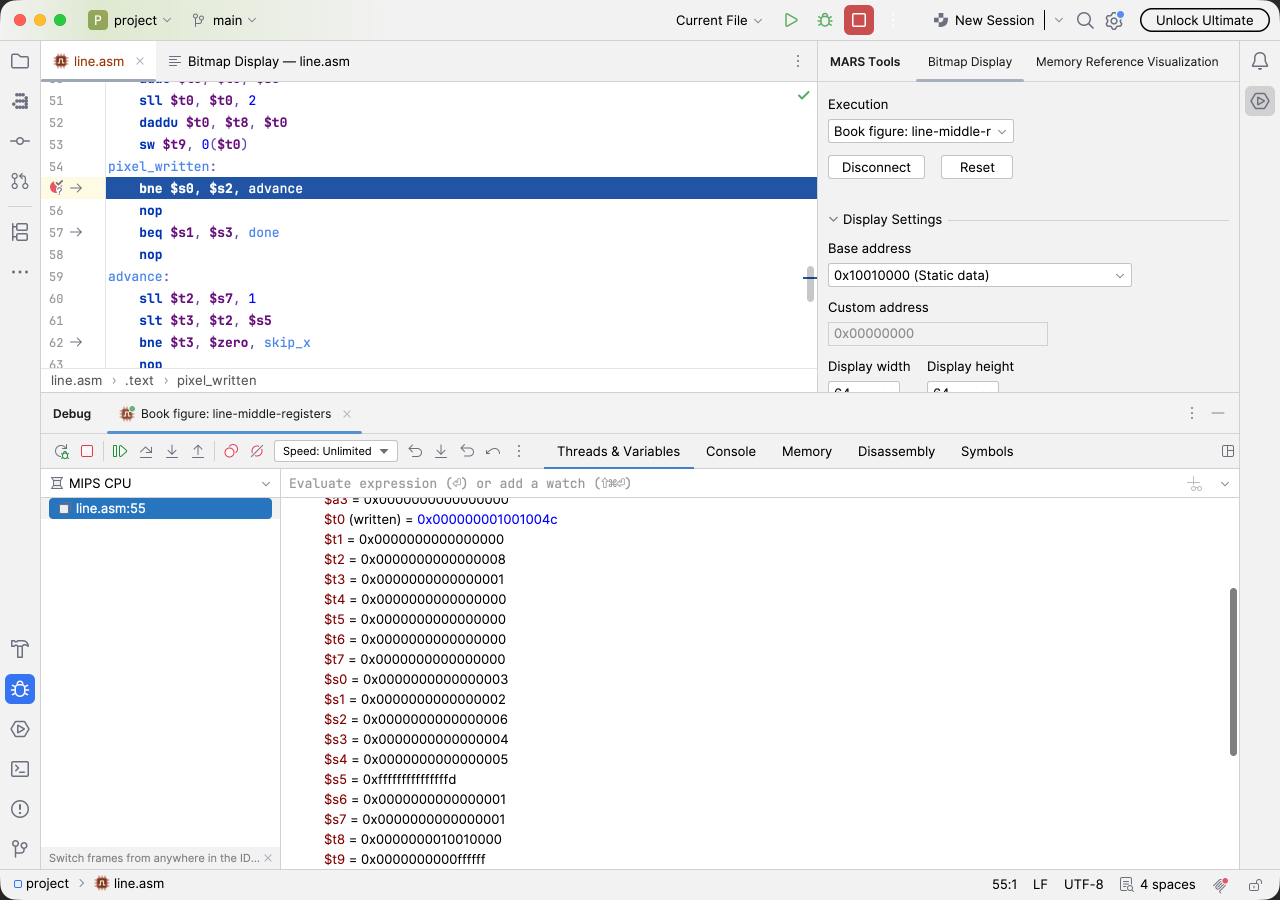
\includegraphics[artifact]{book/captures/007-bresenham-line/f03-middle/registers.png}}
\sbox2{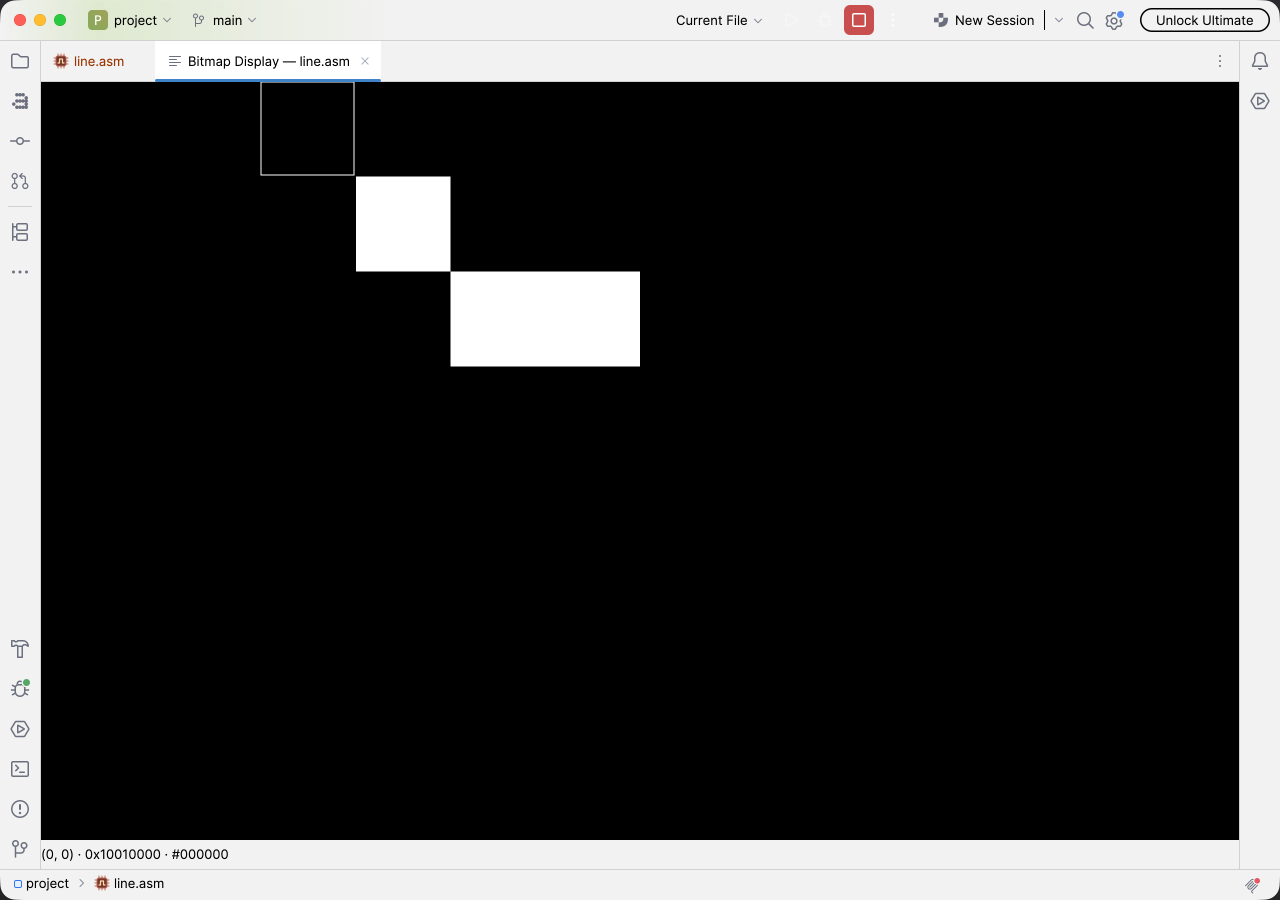
\includegraphics[artifact]{book/captures/007-bresenham-line/f03-middle/bitmap.png}}
\edef\MARSmiddlesourceLeft{\the\dimexpr0.036718750\wd0\relax}
\edef\MARSmiddlesourceBottom{\the\dimexpr0.774444444\ht0\relax}
\edef\MARSmiddlesourceRight{\the\dimexpr0.611718750\wd0\relax}
\edef\MARSmiddlesourceTop{\the\dimexpr0.147777778\ht0\relax}
\edef\MARSmiddlestateLeft{\the\dimexpr0.246093750\wd0\relax}
\edef\MARSmiddlestateBottom{\the\dimexpr0.075555556\ht0\relax}
\edef\MARSmiddlestateRight{\the\dimexpr0.596875000\wd0\relax}
\edef\MARSmiddlestateTop{\the\dimexpr0.740000000\ht0\relax}
\edef\MARSmiddleplotLeft{\the\dimexpr0.203906250\wd2\relax}
\edef\MARSmiddleplotBottom{\the\dimexpr0.066666667\ht2\relax}
\edef\MARSmiddleplotRight{\the\dimexpr0.203906250\wd2\relax}
\edef\MARSmiddleplotTop{\the\dimexpr0.091111111\ht2\relax}
\edef\MARSmiddlesavedLeft{\the\dimexpr0.246093750\wd0\relax}
\edef\MARSmiddlesavedBottom{\the\dimexpr0.364444444\ht0\relax}
\edef\MARSmiddlesavedRight{\the\dimexpr0.599218750\wd0\relax}
\edef\MARSmiddlesavedTop{\the\dimexpr0.606666667\ht0\relax}
\begin{tikzpicture}[alt={Four annotated details at the third pixel written boundary selected by native condition s0 equals three. The bitmap contains white cells one one, two two and three two. Working coordinate is three two and running error is one. Scratch register t2 remains eight from the preceding update; the next doubled-error calculation has not executed.}]
\node[anchor=north west,inner sep=0,font=\small\bfseries] (source-title) at (6mm,0) {The third store is complete};
\node[anchor=north west,inner sep=0] (source) at ([yshift=-1mm]source-title.south west) {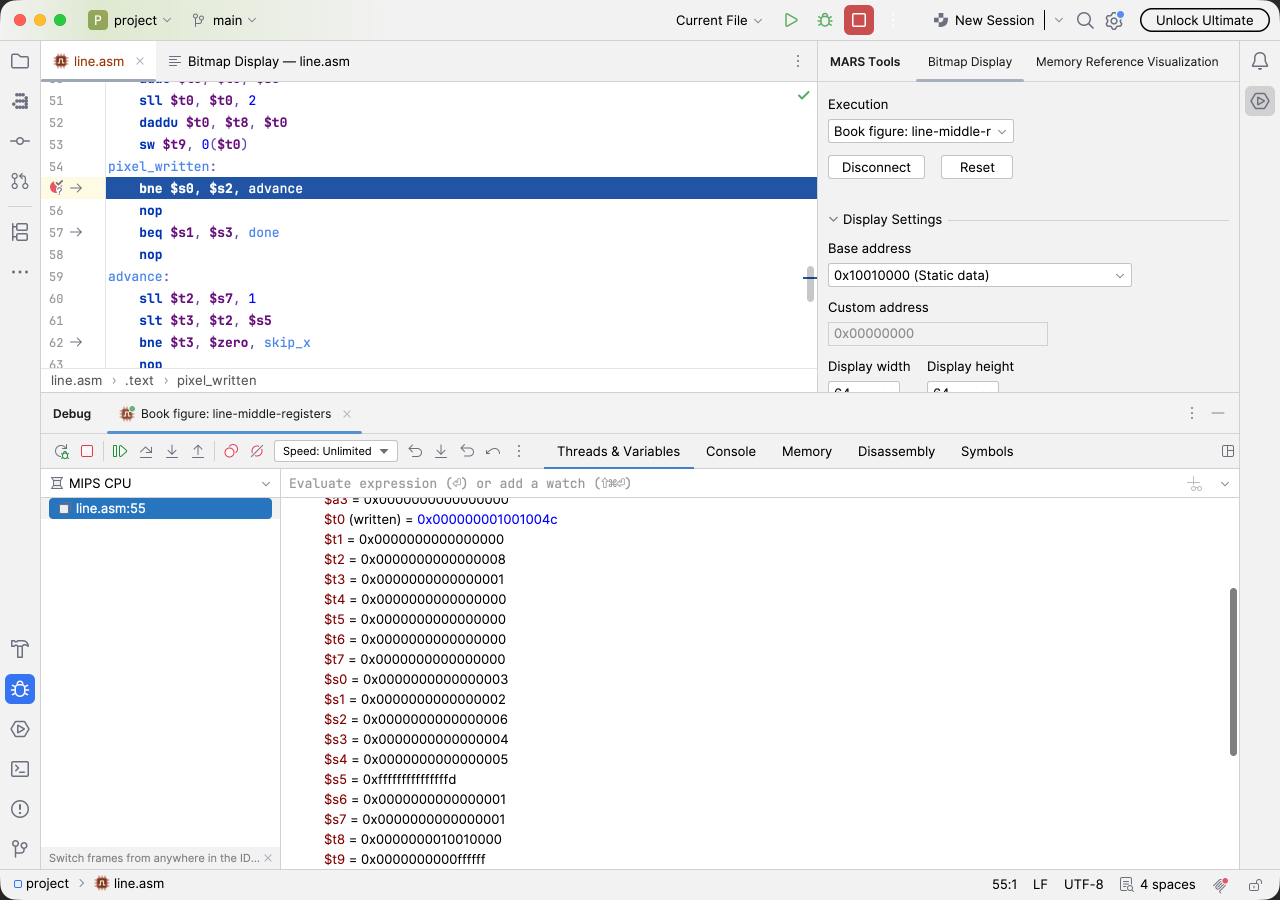
\includegraphics[width=0.7\linewidth,artifact,trim={\MARSmiddlesourceLeft{} \MARSmiddlesourceBottom{} \MARSmiddlesourceRight{} \MARSmiddlesourceTop{}},clip]{book/captures/007-bresenham-line/f03-middle/registers.png}};
\begin{scope}[shift={(source.south west)},x={($(source.south east)-(source.south west)$)},y={($(source.north west)-(source.south west)$)}]
\draw[black,line width=0.7pt] (0.135555556,0.057142857) rectangle (0.568888889,0.371428571);
\node[draw=black,fill=white,circle,inner sep=1.5pt,font=\footnotesize] at ($(0.135555556,0.371428571)+(-3mm,0)$) {1};
\end{scope}
\node[anchor=north west,inner sep=0,font=\small\bfseries] (state-title) at ([yshift=-2mm]source.south west) {The running error has changed to one};
\node[anchor=north west,inner sep=0] (state) at ([yshift=-1mm]state-title.south west) {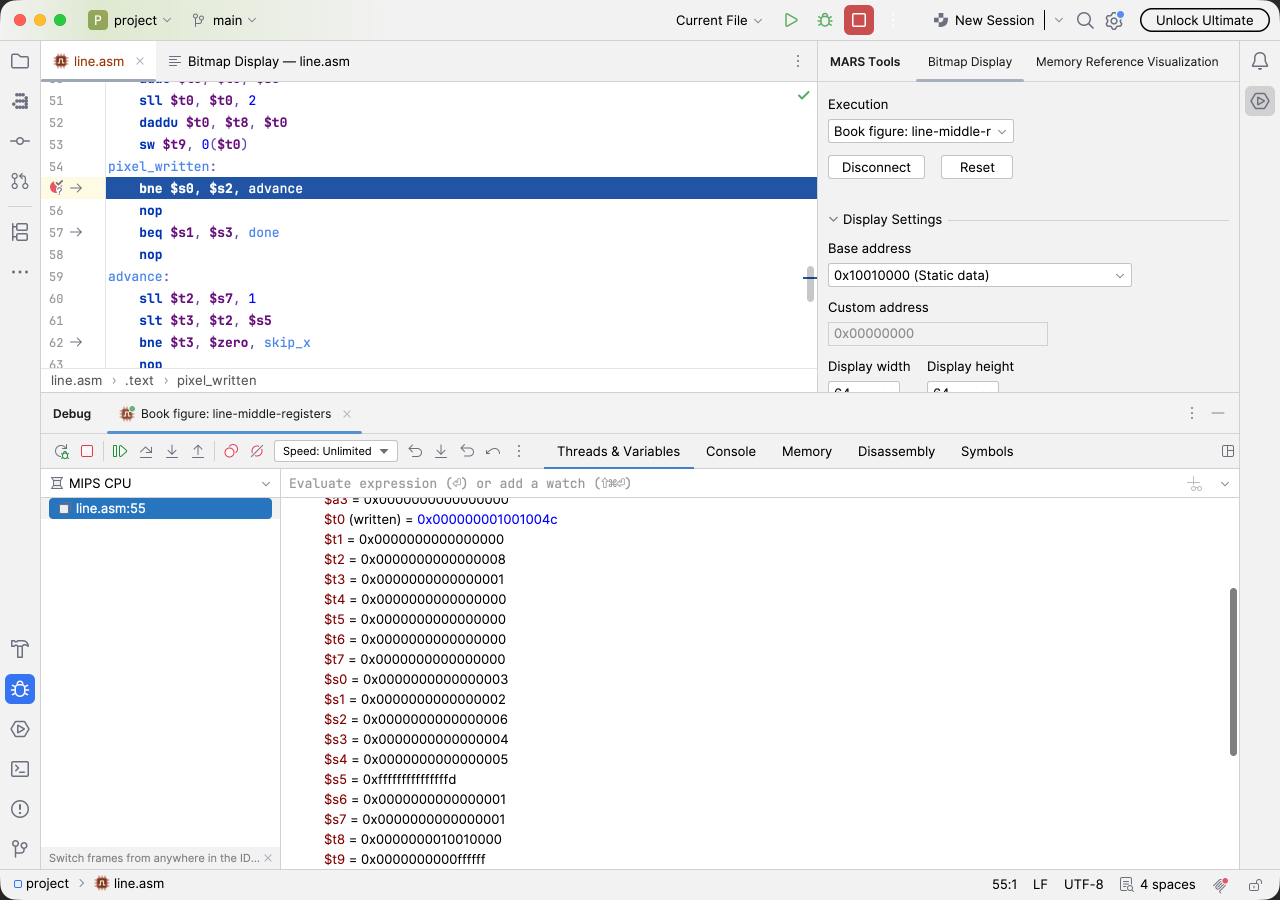
\includegraphics[width=0.4\linewidth,artifact,trim={\MARSmiddlestateLeft{} \MARSmiddlestateBottom{} \MARSmiddlestateRight{} \MARSmiddlestateTop{}},clip]{book/captures/007-bresenham-line/f03-middle/registers.png}};
\begin{scope}[shift={(state.south west)},x={($(state.south east)-(state.south west)$)},y={($(state.north west)-(state.south west)$)}]
\draw[black,line width=0.7pt] (0.029850746,0.018072289) rectangle (0.970149254,0.981927711);
\node[draw=black,fill=white,circle,inner sep=1.5pt,font=\footnotesize] at ($(0.029850746,0.981927711)+(-3mm,0)$) {2};
\end{scope}
\node[anchor=north west,inner sep=0,font=\small\bfseries] (plot-title) at ([xshift=0.49\linewidth]state-title.north west) {Three cells have been painted};
\node[anchor=north west,inner sep=0] (plot) at ([yshift=-1mm]plot-title.south west) {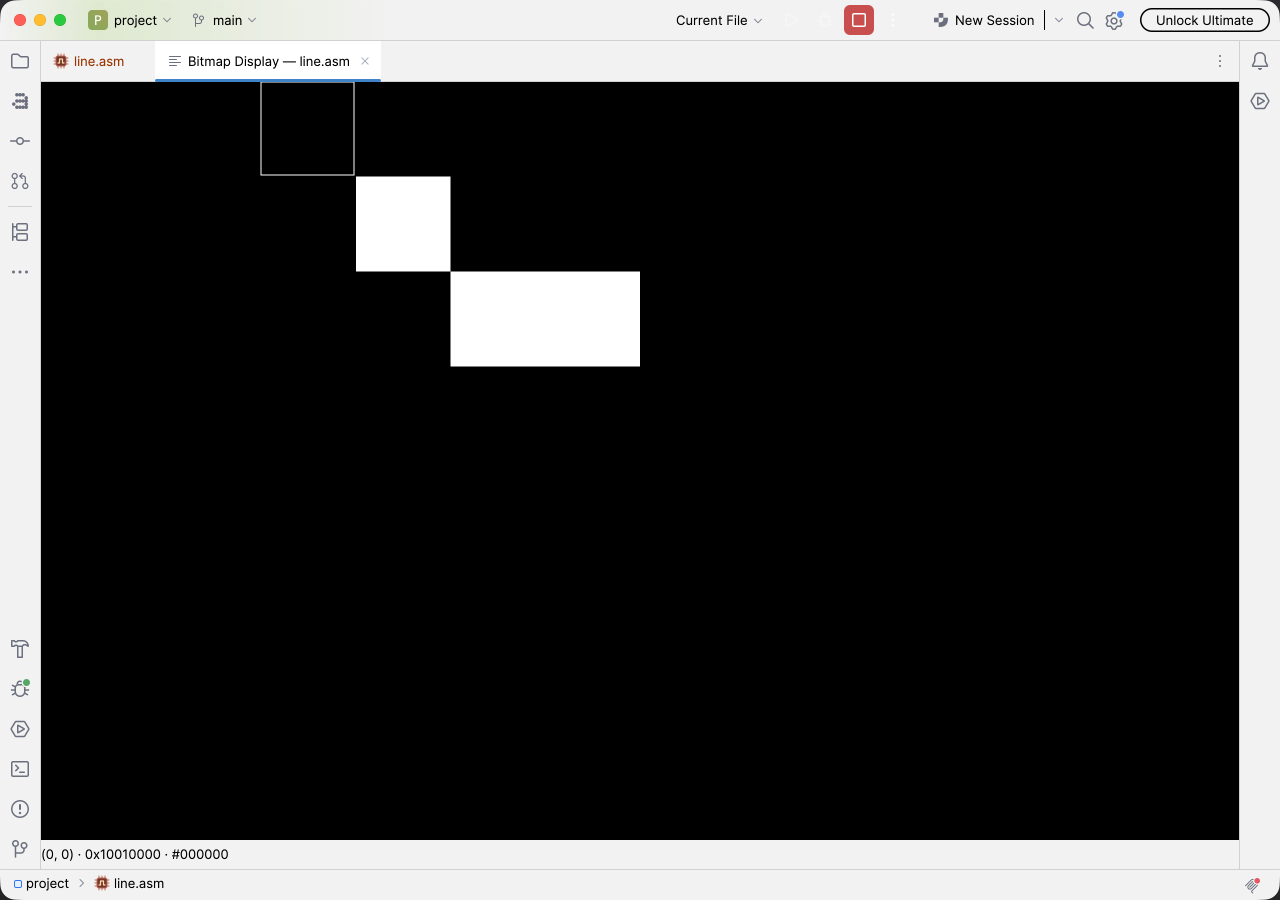
\includegraphics[width=0.32\linewidth,artifact,trim={\MARSmiddleplotLeft{} \MARSmiddleplotBottom{} \MARSmiddleplotRight{} \MARSmiddleplotTop{}},clip]{book/captures/007-bresenham-line/f03-middle/bitmap.png}};
\begin{scope}[shift={(plot.south west)},x={($(plot.south east)-(plot.south west)$)},y={($(plot.north west)-(plot.south west)$)}]
\draw[black,line width=0.7pt] (0.000000000,0.000000000) rectangle (1.000000000,1.000000000);
\node[draw=black,fill=white,circle,inner sep=1.5pt,font=\footnotesize] at ($(0.000000000,1.000000000)+(-3mm,0)$) {3};
\foreach \c in {0,...,7} {\node[anchor=north,font=\scriptsize,inner sep=0] at ({(\c+0.5)/8},-0.035) {\c}; \node[anchor=east,font=\scriptsize,inner sep=0] at (-0.025,{1-(\c+0.5)/8}) {\c};}
\node[anchor=north,font=\scriptsize,inner sep=0] at (0.5,-0.11) {$x$}; \node[anchor=east,font=\scriptsize,inner sep=0] at (-0.10,0.5) {$y$};
\end{scope}
\node[anchor=north west,inner sep=0,font=\small\bfseries] (saved-title) at ([yshift=-2mm]state.south west) {A scratch register retains the prior decision};
\node[anchor=north west,inner sep=0] (saved) at ([yshift=-1mm]saved-title.south west) {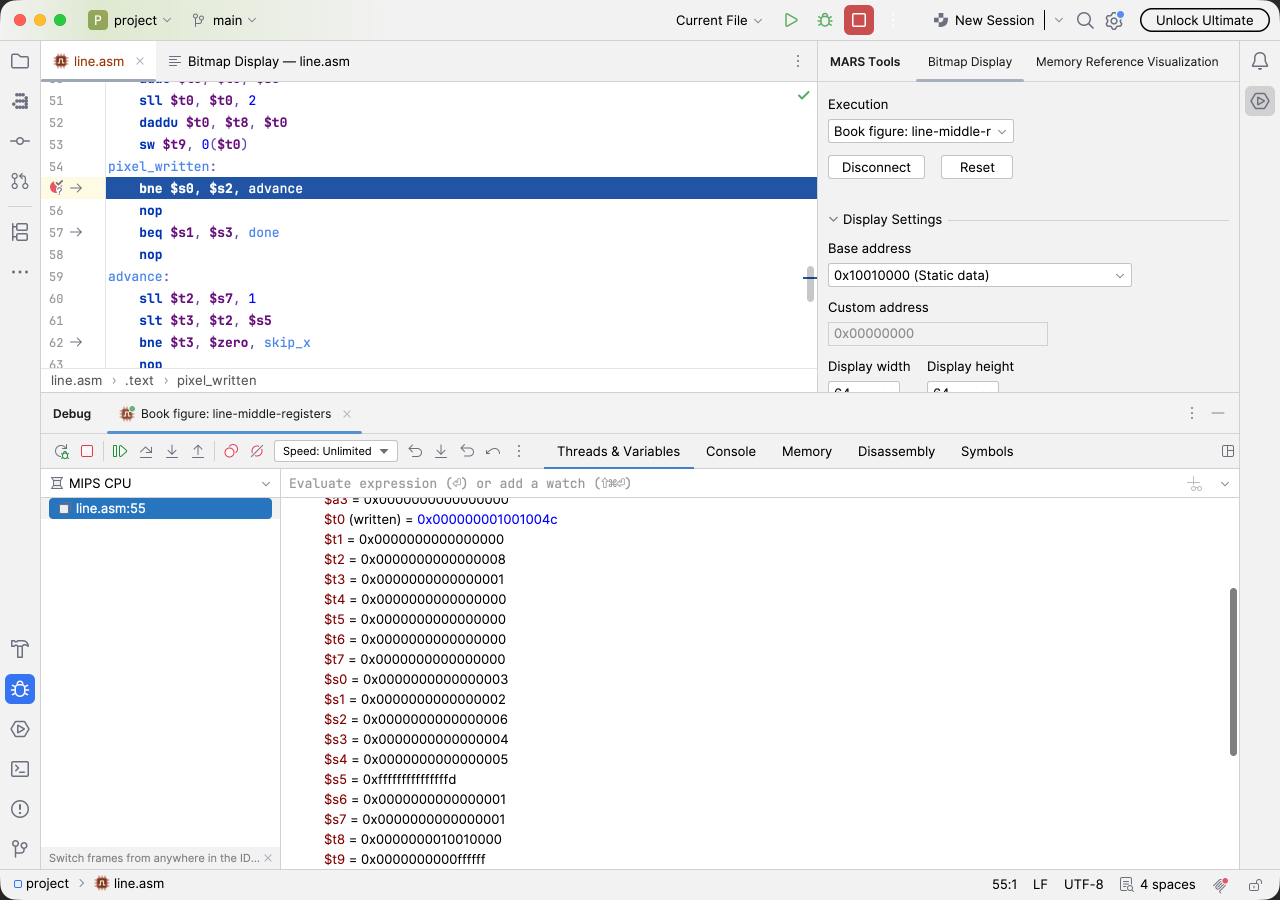
\includegraphics[width=0.4\linewidth,artifact,trim={\MARSmiddlesavedLeft{} \MARSmiddlesavedBottom{} \MARSmiddlesavedRight{} \MARSmiddlesavedTop{}},clip]{book/captures/007-bresenham-line/f03-middle/registers.png}};
\begin{scope}[shift={(saved.south west)},x={($(saved.south east)-(saved.south west)$)},y={($(saved.north west)-(saved.south west)$)}]
\draw[black,line width=0.7pt] (0.030303030,0.115384615) rectangle (0.969696970,0.884615385);
\node[draw=black,fill=white,circle,inner sep=1.5pt,font=\footnotesize] at ($(0.030303030,0.884615385)+(-3mm,0)$) {4};
\end{scope}
\end{tikzpicture}
\par\smallskip
\begin{minipage}{\linewidth}
\small
\begin{enumerate}
\item A native breakpoint condition, \texttt{\$s0 == 3}, selects this occurrence of \texttt{pixel\_written}. The store at $(3,2)$ has executed; the blue endpoint test has not.
\item The previous sample was $(2,2)$ with error 4. The x update adds $dy=-3$, leaving error 1 and coordinate $(3,2)$. The y update was skipped, so y remains 2.
\item The white cells are $(1,1)$, $(2,2)$ and $(3,2)$. The adjacent cells in row 2 result from the decision to advance x alone. All other framebuffer words retain their initial zero value.
\item \texttt{\$t2}=8 came from doubling the previous error 4. It passed the x test and failed the y test because $8>dx=5$. At this pause it is not twice the current error 1. A later \texttt{sll} will replace it with 2 if the loop advances again.
\end{enumerate}
\end{minipage}
\caption{The third sample follows an update that changed x alone. The saved doubled error still belongs to the previous decision cycle.}
\label{capture:007-bresenham-line-f03-middle}
\end{figure}
\par
